\documentclass[aspectratio=169,11pt]{beamer}

\usetheme{Madrid}
\usecolortheme{default}
\usefonttheme{professionalfonts}
\setbeamertemplate{navigation symbols}{}
\setbeamertemplate{footline}[frame number]

\usepackage{amsmath, amssymb, booktabs, graphicx}
\graphicspath{{../../assets/figures/}{assets/figures/}}

\title{Technology, Automation, AI, and Labor Market}
\subtitle{Labor II --- Week 11}
\author{Teaching deck draft}
\date{}

\begin{document}

\begin{frame}
  \titlepage
\end{frame}

\begin{frame}{Central question and course repositioning}
\begin{itemize}
    \item How do technology, automation, and AI reshape work through worker adaptation, firm labor demand, and market-level reallocation?
    \item Week 11 is a major shock-and-adjustment lecture, not a generic AI detour.
    \item The labor-market objects stay familiar: tasks, employment, wages, vacancies, worker learning, and equilibrium incidence.
\end{itemize}
\end{frame}

\begin{frame}{Week 10 to Week 11 bridge}
\begin{itemize}
    \item Week 10: cyclical shocks moved unemployment, vacancies, separations, mobility, and match quality.
    \item Week 11: technology shocks move many of the same margins, but through more persistent restructuring.
    \item Week 12 will then shift from technology shocks inside production to trade and offshoring shocks through global integration.
\end{itemize}
\end{frame}

\begin{frame}{Why technology is not just a labor-demand topic}
\begin{itemize}
    \item Supply side: learning, retraining, search/application technology, and skill obsolescence.
    \item Demand side: automation, augmentation, vacancy redesign, and workforce composition.
    \item Market level: local reallocation, labor-share shifts, wage incidence, and cross-place spillovers.
\end{itemize}
\end{frame}

\begin{frame}{Supply, demand, and market-level feedbacks}
\begin{center}
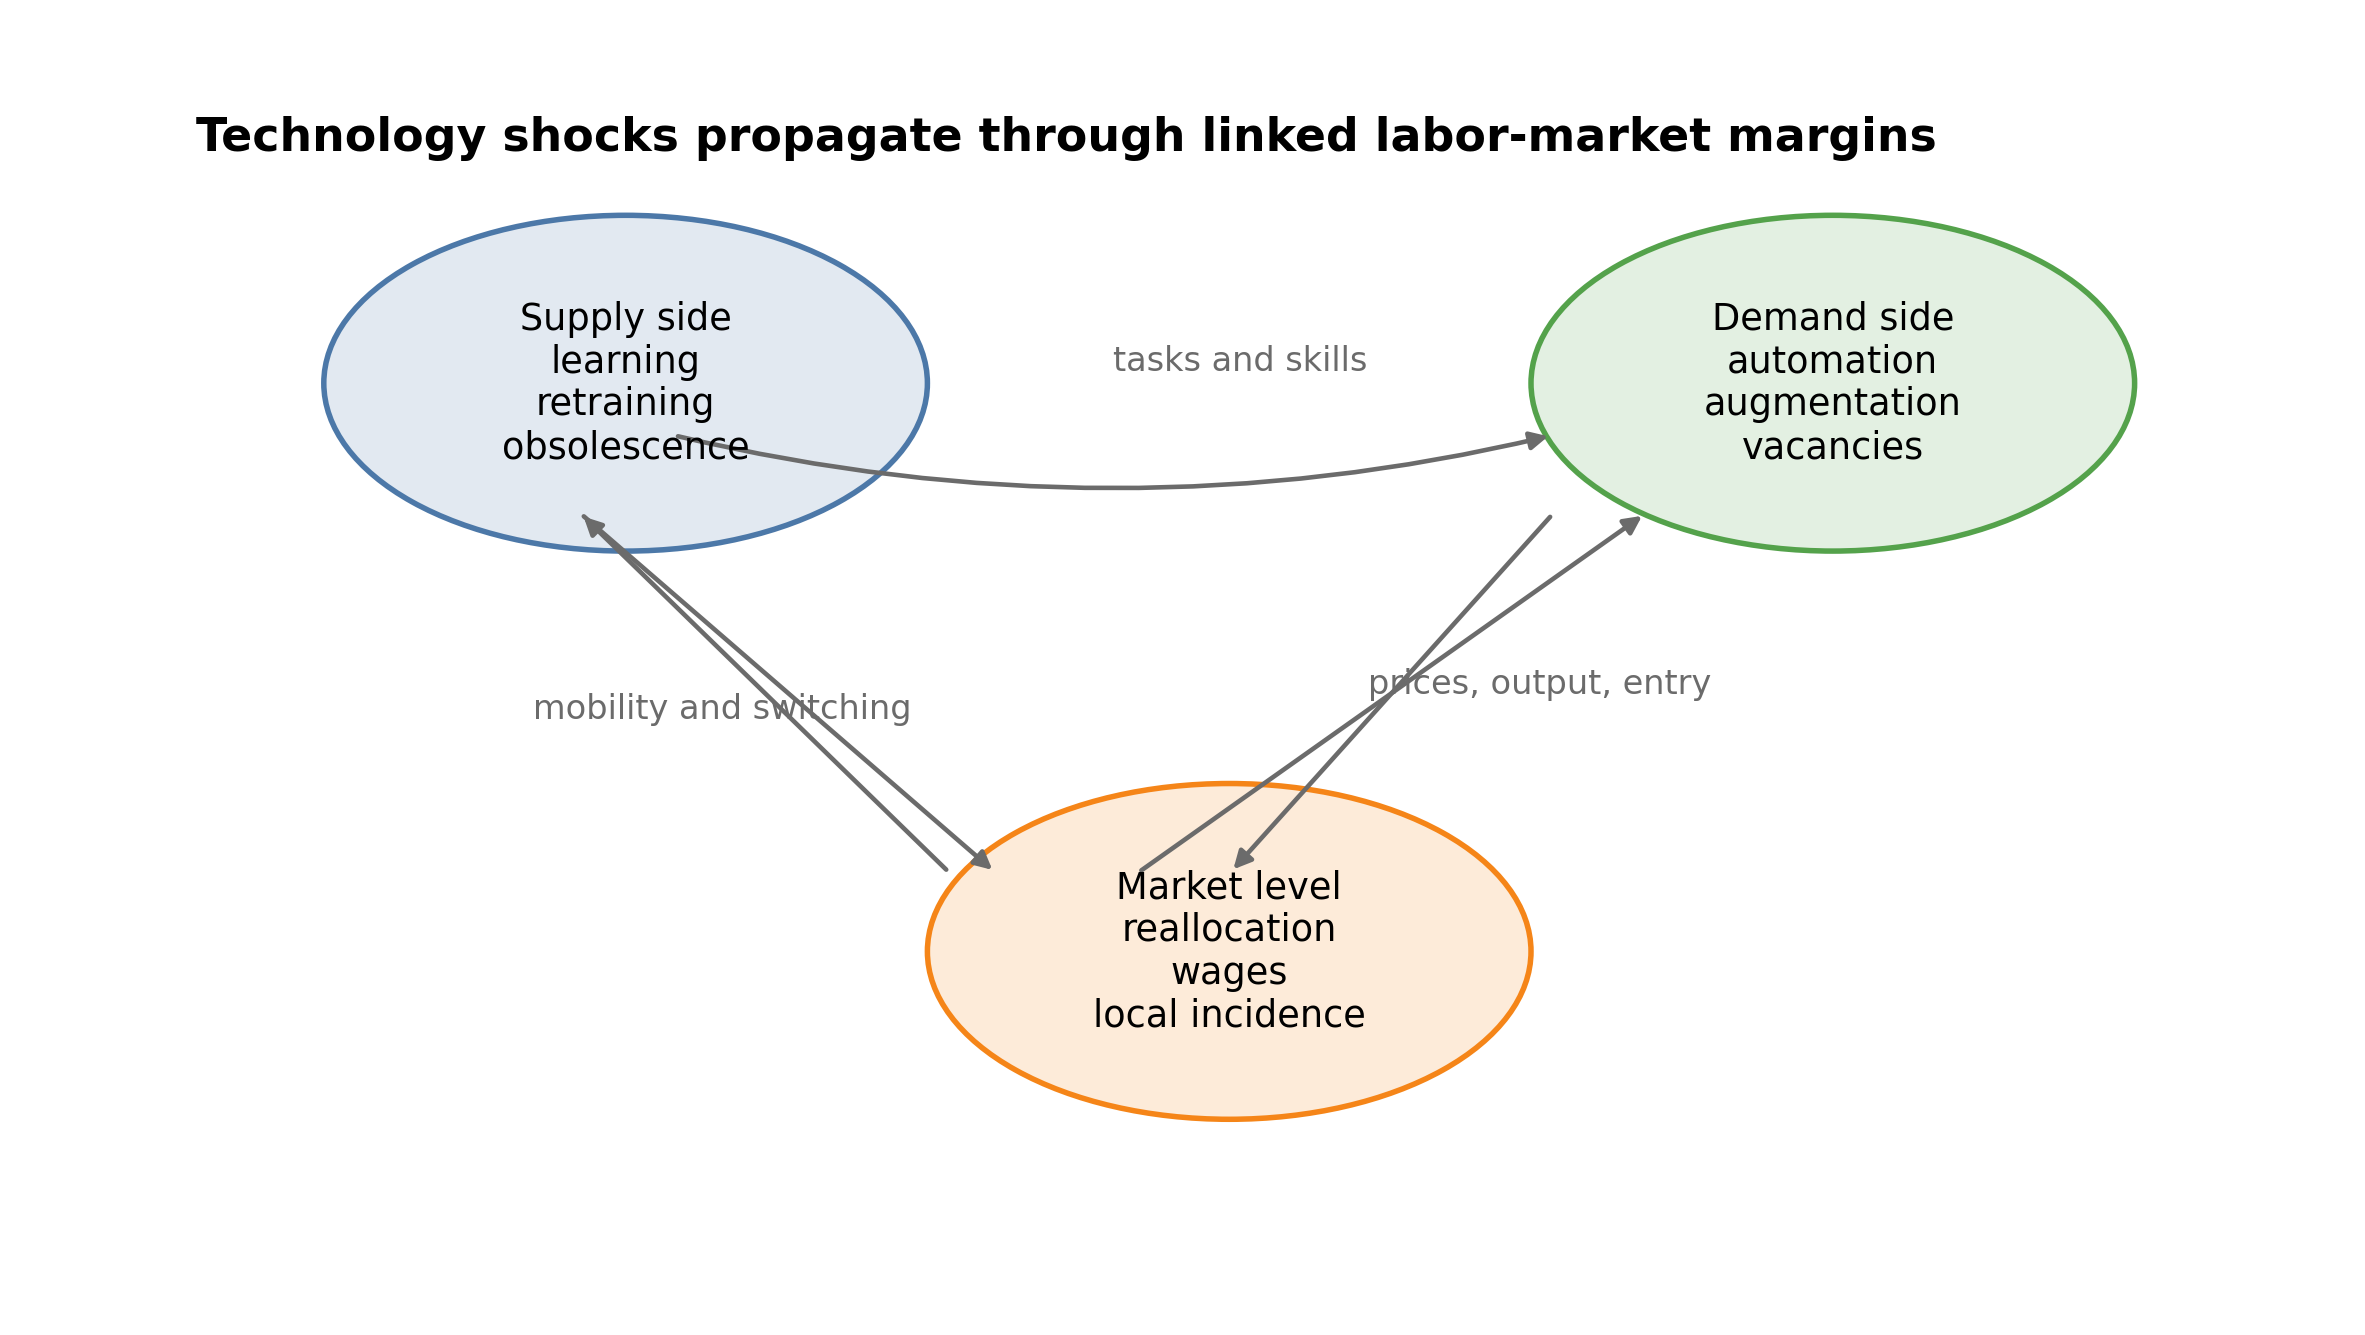
\includegraphics[height=0.73\textheight]{11-supply-demand-market-effects.png}
\end{center}
\end{frame}

\begin{frame}{Task-based framework: automation, augmentation, and new tasks}
\begin{center}
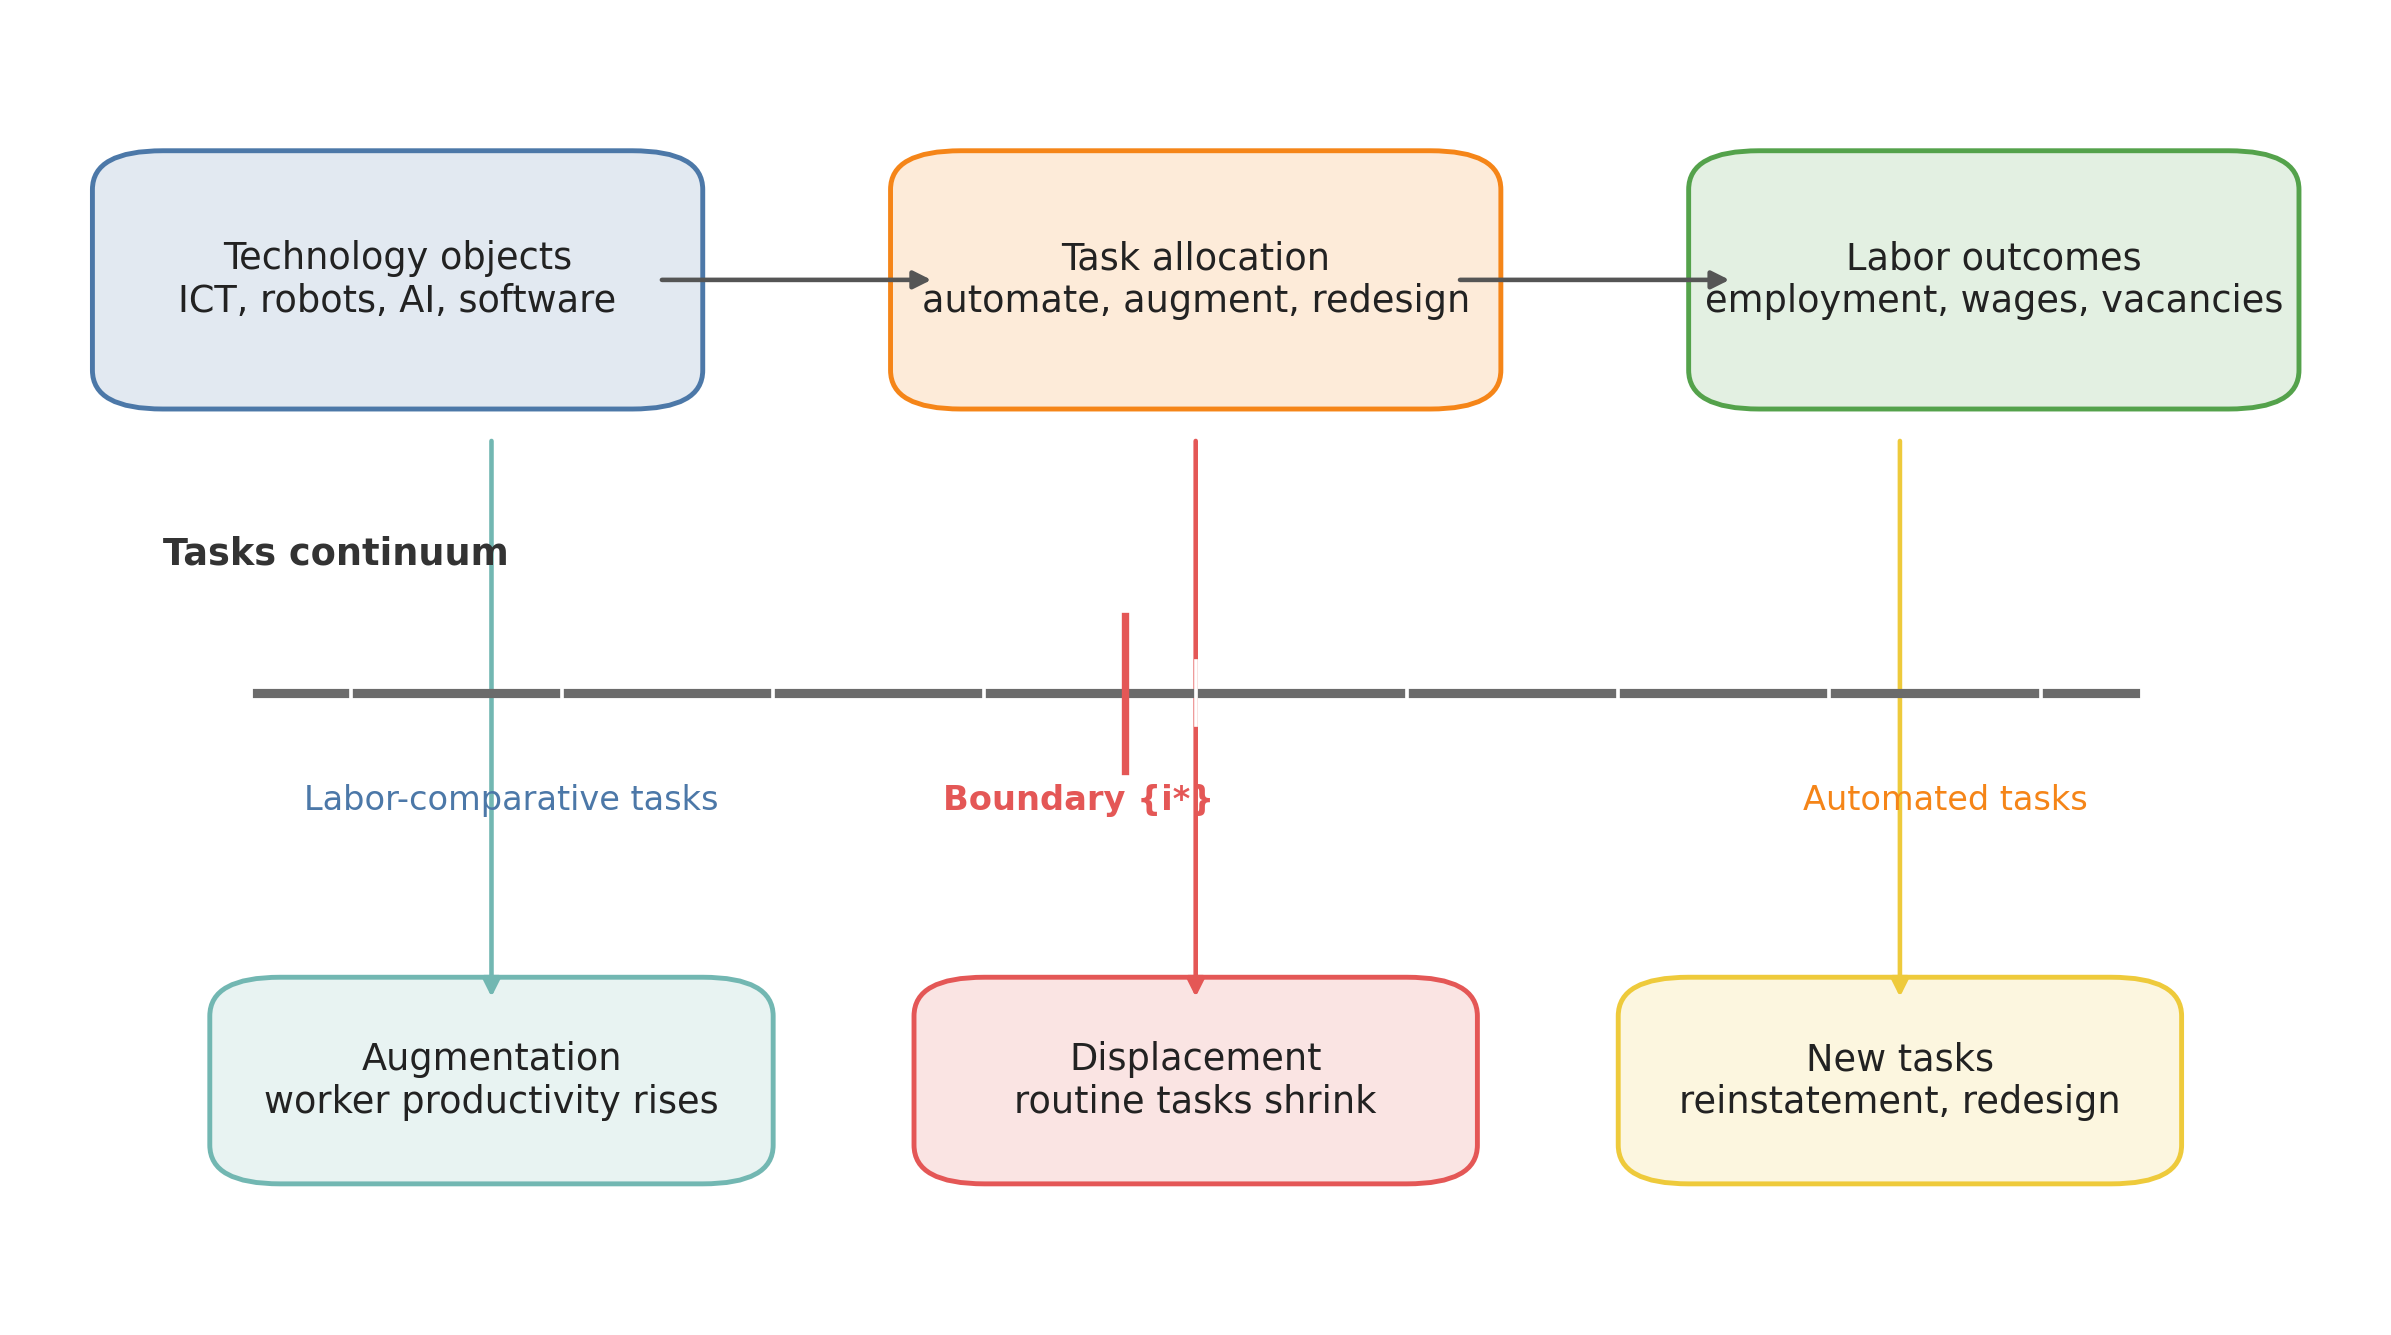
\includegraphics[height=0.72\textheight]{11-task-based-technology-framework.png}
\end{center}
\end{frame}

\begin{frame}{One task-based production object}
\[
Y_t =
\left[\int_0^1 y_t(i)^{\frac{\sigma-1}{\sigma}} \, di \right]^{\frac{\sigma}{\sigma-1}}
\]

\begin{itemize}
    \item Tasks, not occupations, are the primitive object.
    \item Technology changes task productivity and the elasticity of reallocation across tasks.
    \item Observed occupations are bundles of tasks with changing internal content.
\end{itemize}
\end{frame}

\begin{frame}{Automation boundary and task allocation}
\[
\frac{w_t}{a_t(i_t^\ast)} = \frac{c_t^{T}}{b_t(i_t^\ast)},
\qquad
\mathcal{A}_t = \left\{i : \frac{c_t^{T}}{b_t(i)} \le \frac{w_t}{a_t(i)} \right\}
\]

\begin{itemize}
    \item Lower technology cost or higher machine productivity expands the automated task set.
    \item That shift does not by itself reveal the sign of aggregate labor-demand effects.
    \item Productivity, output expansion, and new tasks can offset direct displacement.
\end{itemize}
\end{frame}

\begin{frame}{Displacement, productivity, and reinstatement}
\[
\Delta \log L_t =
\Delta \log L_t^{disp}
+
\Delta \log L_t^{prod}
+
\Delta \log L_t^{new}
\]

\begin{itemize}
    \item Direct substitution is only one term in the labor-demand accounting.
    \item Empirically, students should ask which term a paper is closest to observing.
    \item Market-level incidence depends on all three channels plus reallocation frictions.
\end{itemize}
\end{frame}

\begin{frame}{Supply-side adjustment: learning, training, and obsolescence}
\[
H_{t+1} = (1-\delta_t)H_t + I_t
\]

\begin{itemize}
    \item Technology can raise the payoff to learning while increasing skill obsolescence.
    \item Worker-side adjustment is not just schooling; it includes on-the-job learning and occupational switching.
    \item Productivity gains for some workers need not imply welfare gains for all workers.
\end{itemize}
\end{frame}

\begin{frame}{Historical perspective: ICT, polarization, and long-run adjustment}
\begin{itemize}
    \item Autor: labor demand did not disappear because technology also created complementary and new tasks.
    \item Acemoglu-Restrepo: automation displaces labor, but reinstatement matters.
    \item Michaels-Natraj-Van Reenen: ICT shifted demand toward high-skill tasks and away from routine middle-skill work.
\end{itemize}
\end{frame}

\begin{frame}{Demand-side evidence: robots, ICT, AI adoption, and vacancies}
\begin{itemize}
    \item Robots: local-labor-market exposure captures wage and employment incidence across places.
    \item Cross-country robot panels capture broad productivity and labor-share patterns.
    \item Vacancy data reveal changing task content and hiring intent, not realized employment by themselves.
    \item Firm adoption data are closer to treatment, but selection into adoption is central.
\end{itemize}
\end{frame}

\begin{frame}{Market-level equilibrium and reallocation}
\begin{center}
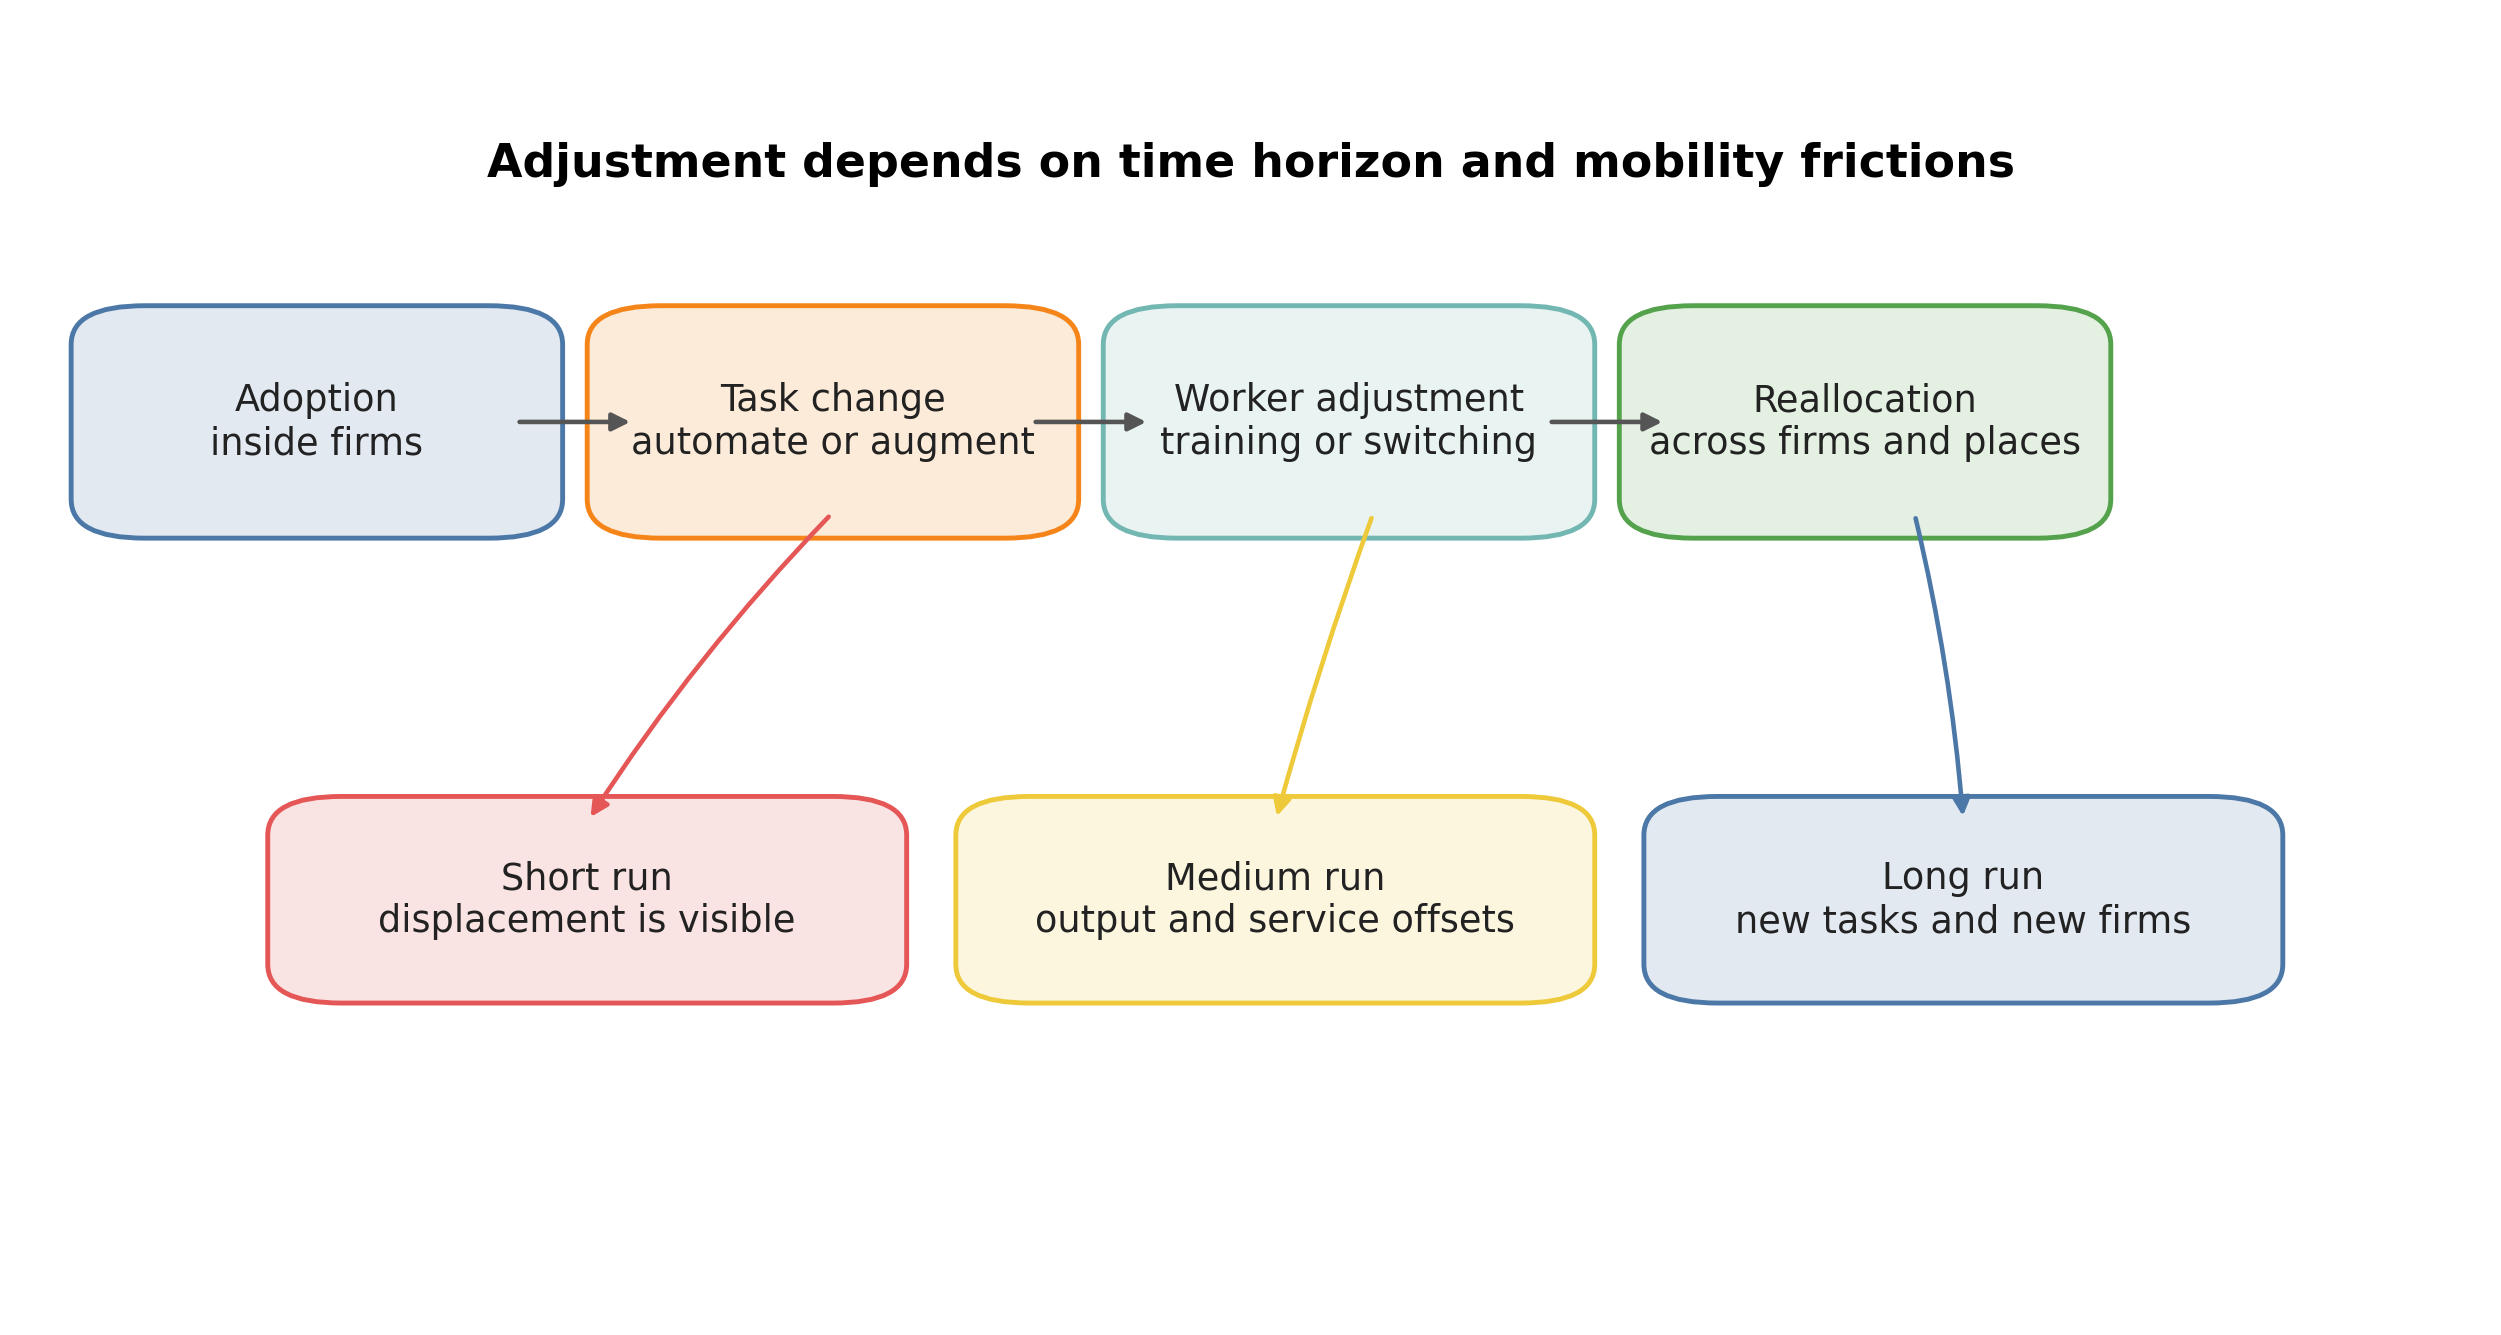
\includegraphics[height=0.72\textheight]{11-technology-adjustment-and-reallocation.png}
\end{center}
\end{frame}

\begin{frame}{Contemporary AI evidence}
\begin{itemize}
    \item Felten-Raj-Seamans: occupation-level AI exposure is a descriptive susceptibility measure.
    \item Acemoglu-Autor-Hazell-Restrepo: online vacancies show changing demand and task content.
    \item Aghion et al.: different uses of AI inside firms can produce different labor-demand responses.
    \item Brynjolfsson-Li-Raymond: worker productivity effects are not the same object as market-level employment effects.
\end{itemize}
\end{frame}

\begin{frame}{Historical and global evidence map}
\begin{center}
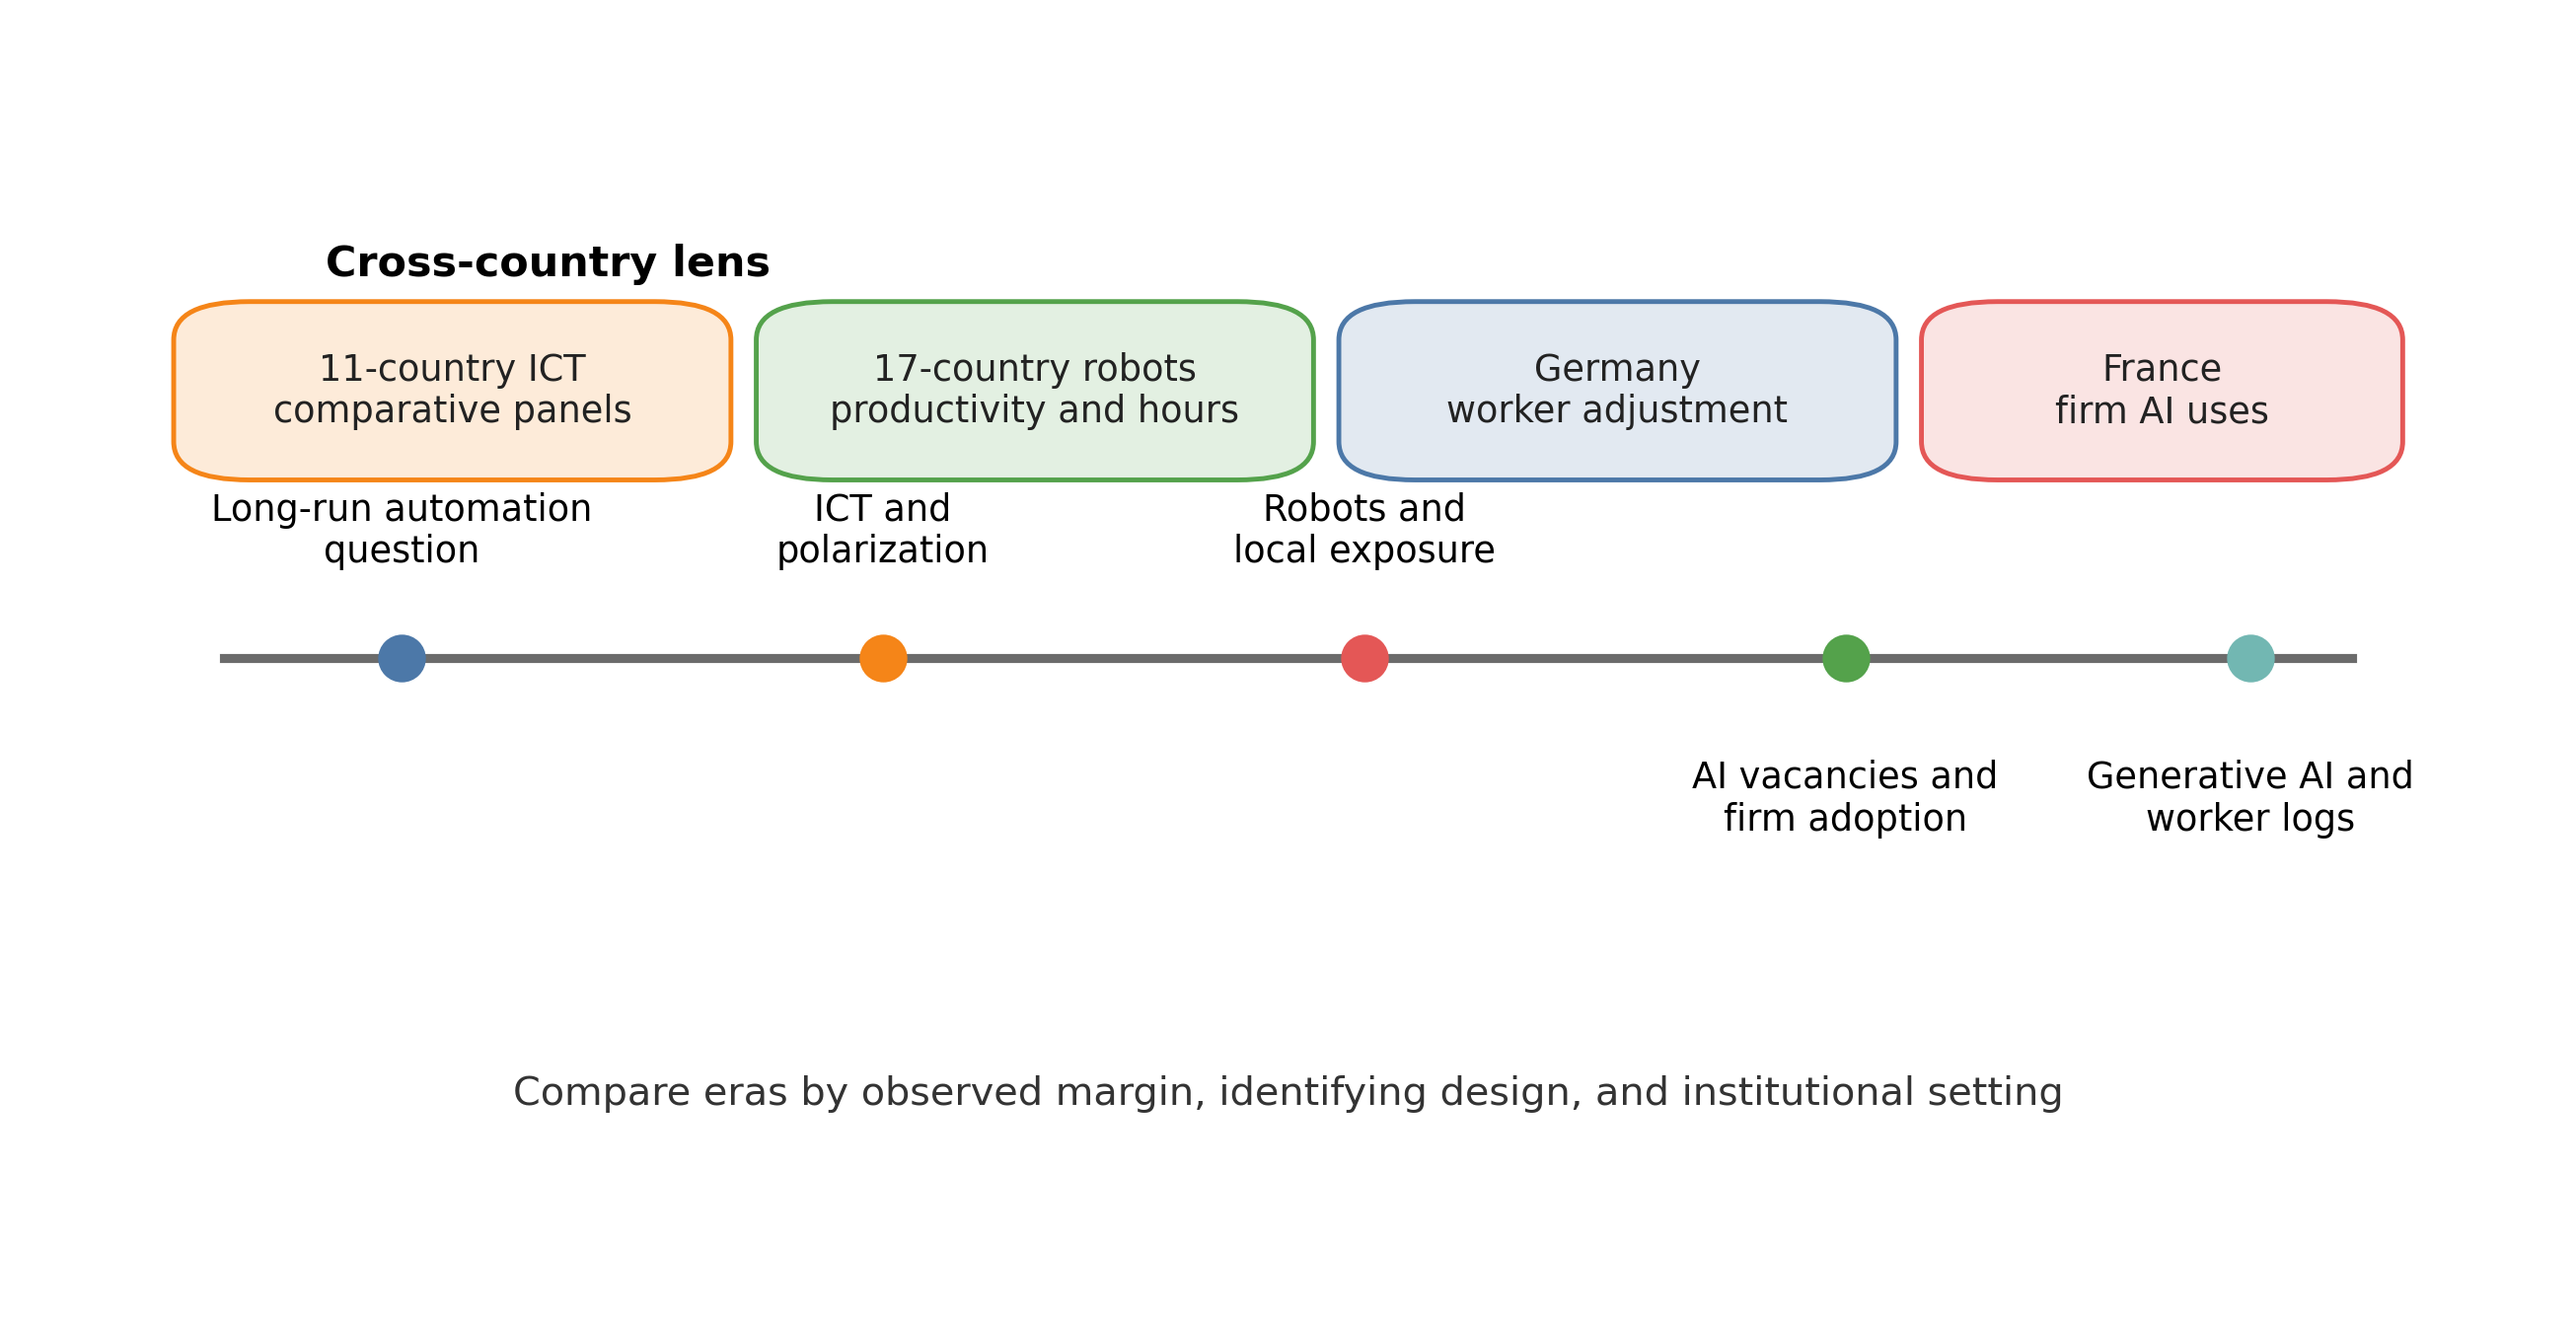
\includegraphics[height=0.71\textheight]{11-historical-global-technology-evidence.png}
\end{center}
\end{frame}

\begin{frame}{AI data and labor-market measurement}
\begin{center}
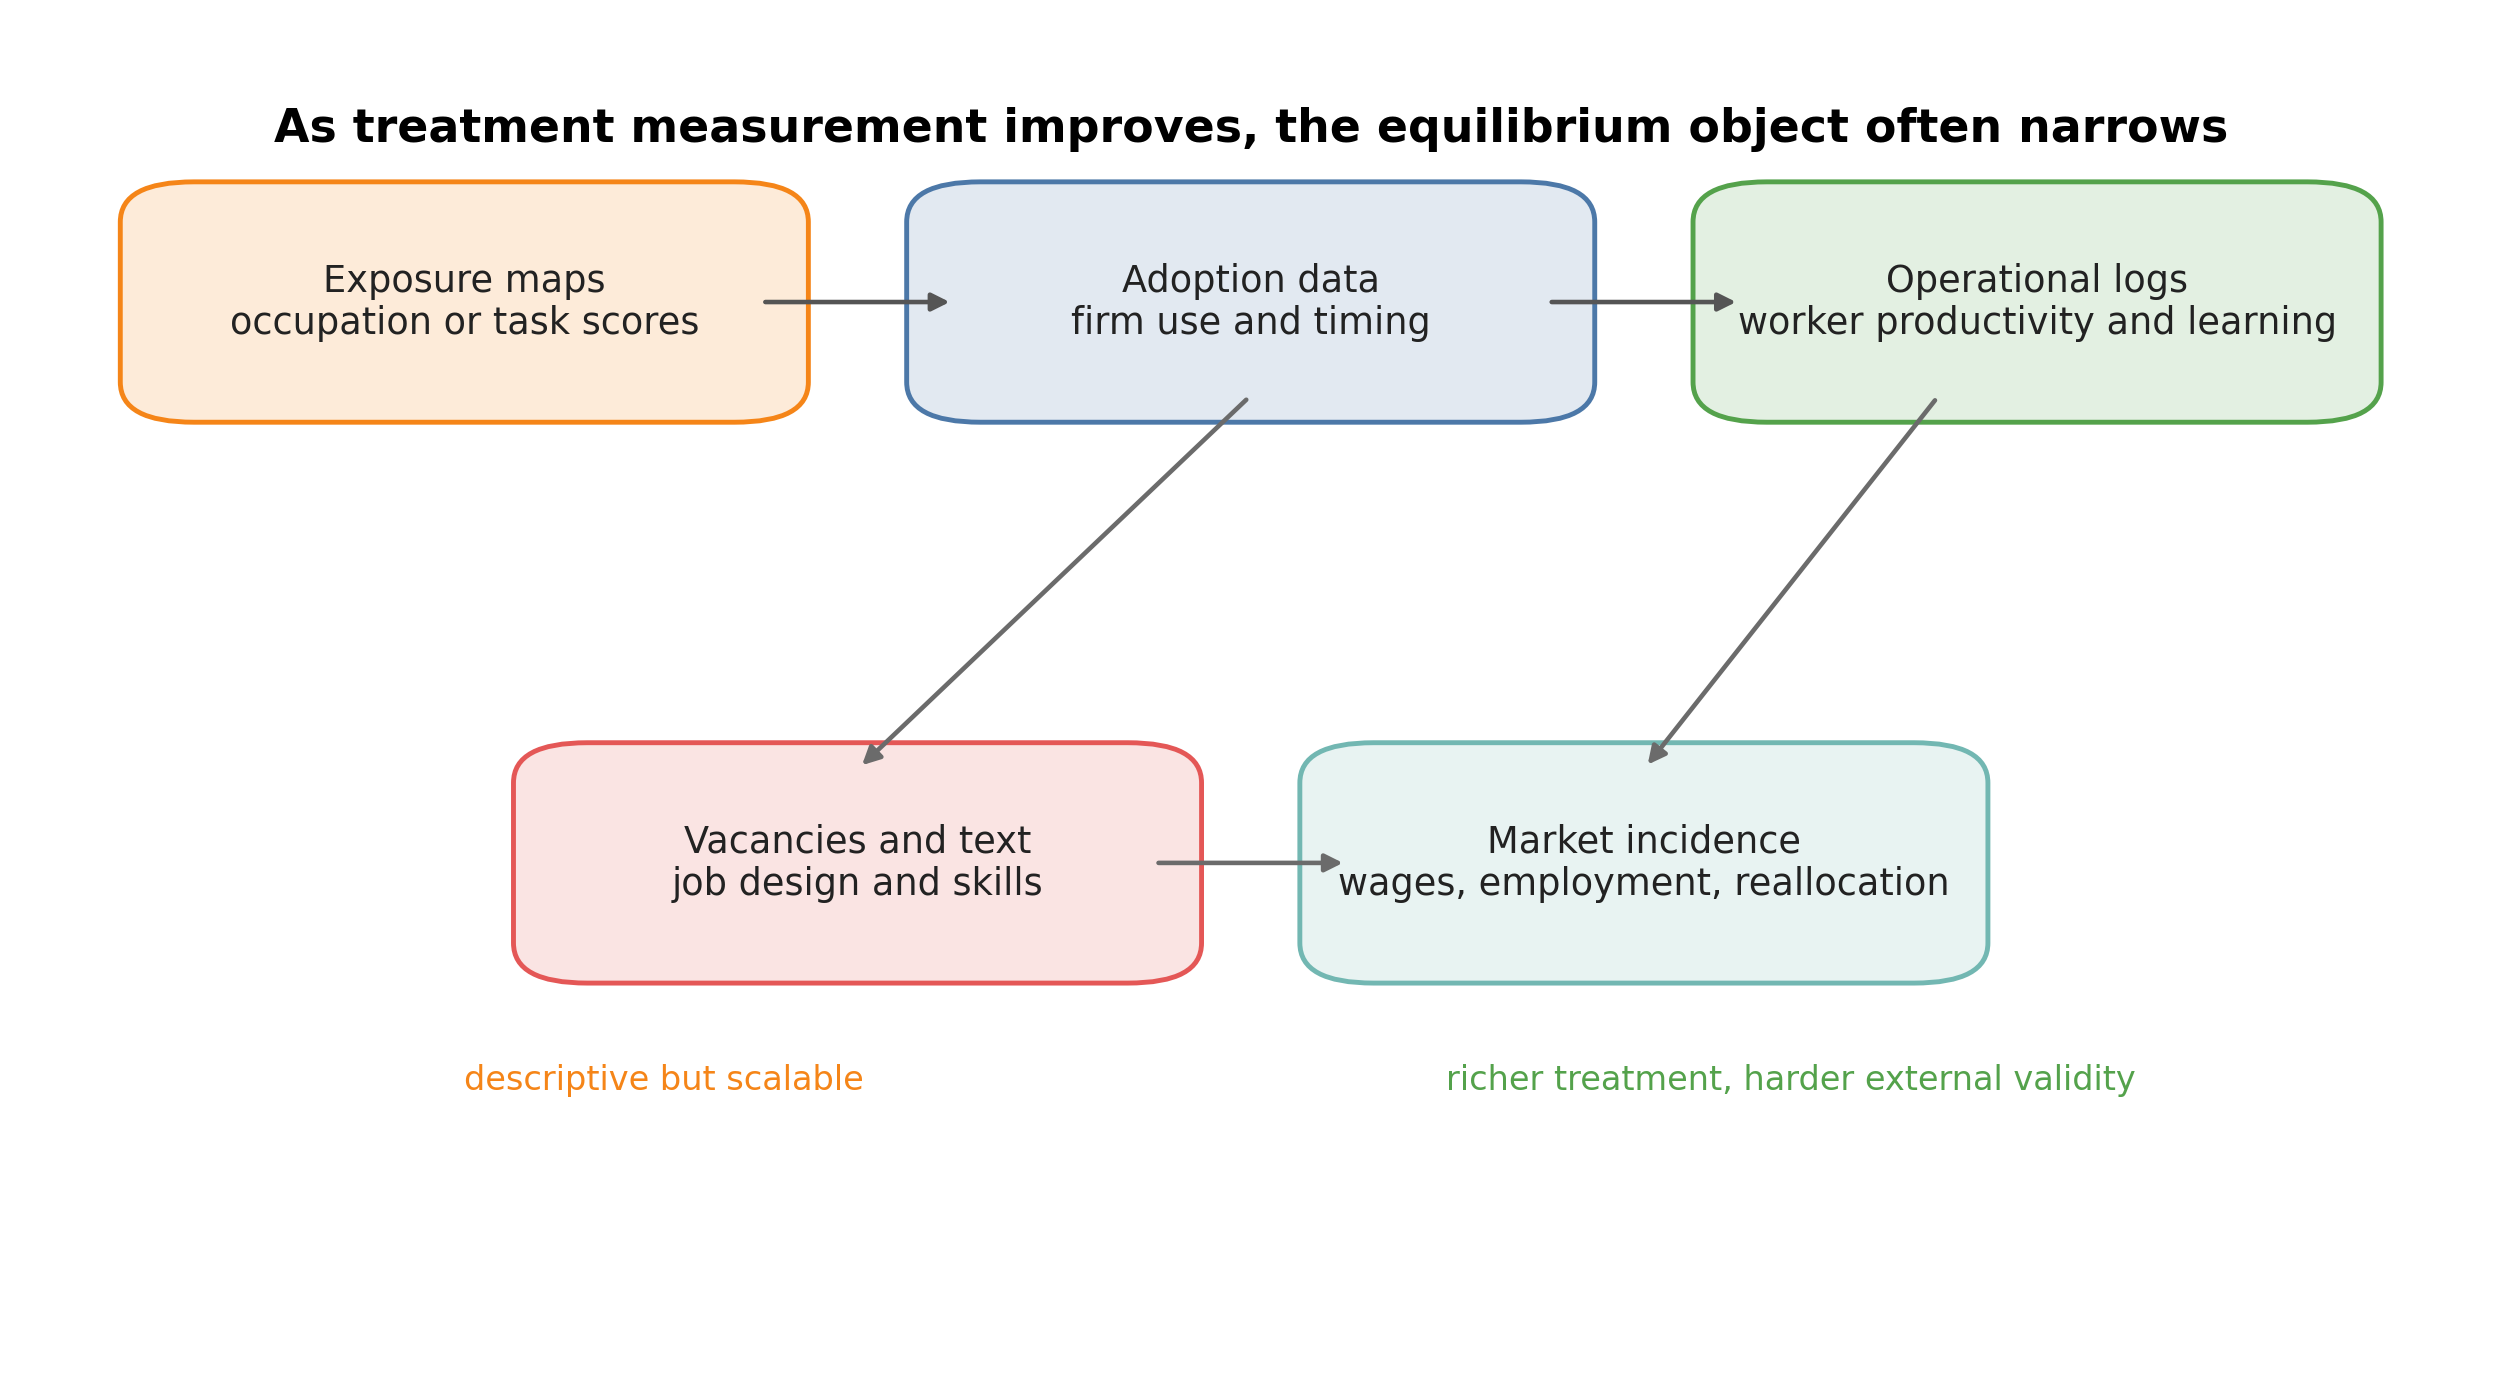
\includegraphics[height=0.71\textheight]{11-ai-data-and-labor-market-measurement.png}
\end{center}
\end{frame}

\begin{frame}{Reduced-form exposure equation and design discipline}
\[
\Delta Y_{mt} = \beta \, TechExposure_{mt} + X_{mt}'\Gamma + \varepsilon_{mt}
\]

\begin{itemize}
    \item Ask whether the technology object is exposure or realized adoption.
    \item Ask whether the unit is a worker, firm, occupation, industry, or local market.
    \item Ask which labor margin is observed and which equilibrium margin stays offstage.
\end{itemize}
\end{frame}

\begin{frame}{Historical evidence versus very recent AI evidence}
\begin{itemize}
    \item ICT and robots come with longer diffusion horizons and clearer realized capital adoption objects.
    \item Very recent AI evidence has stronger exposure measures and faster-moving firm narratives than long-run outcome data.
    \item Students should avoid narrating descriptive exposure maps as if they were already causal adoption evidence.
\end{itemize}
\end{frame}

\begin{frame}{Frontier research questions}
\begin{itemize}
    \item Exposure versus adoption measurement
    \item AI and worker-side search/application technology
    \item Organizational complements and the productivity J-curve
    \item Technology, wage-setting, rent sharing, and labor share
    \item Gender, inequality, and place-based incidence
    \item Training, diffusion policy, and worker transition support
\end{itemize}
\end{frame}

\begin{frame}{Bridge to Week 12 trade and offshoring}
\begin{itemize}
    \item Week 11: shocks begin inside production, task choice, and organizational redesign.
    \item Week 12: shocks begin through global integration, import competition, and offshoring.
    \item Both weeks are about labor-market adjustment, but the mapping from exposure to incidence differs.
\end{itemize}
\end{frame}

\begin{frame}{Takeaways}
\begin{itemize}
    \item Technology is not just a labor-demand topic; it is a supply, demand, and equilibrium topic.
    \item Tasks are more primitive than occupations for theory and measurement.
    \item Exposure, adoption, within-firm evidence, and market-level incidence are distinct objects.
    \item The core empirical challenge is to separate displacement from productivity, new-task, and reallocation effects.
\end{itemize}
\end{frame}

\appendix

\begin{frame}{Appendix: Week 11 lab bridge}
\begin{itemize}
    \item Reproduce: a bounded firm-level AI-use design inspired by Aghion et al.
    \item Diagnose: adoption versus exposure and which margin is actually observed.
    \item Transfer: move one exposure idea to a small synthetic market-level setting.
    \item Challenge extension: contrast within-firm AI evidence with a robot-style local-labor-market design.
\end{itemize}
\end{frame}

\end{document}
